% Copyright 2026 Sreeram Anil
% SPDX-License-Identifier: CC-BY-4.0
\chapter{Cell-level results on the electrochemical plant}
\label{ch:res-cell_spm}

\section{A different kind of test}

The equivalent-circuit results of \cref{ch:res-cell_ecm} measure how well each estimator handles
sensor faults, wrong parameters and wrong initial conditions when the \emph{structure} of its
model is right. The electrochemical benchmark removes that assumption. The truth is now the
single-particle model of \cref{ch:spm} --- solid-phase diffusion in two electrodes,
Butler--Volmer kinetics, an ohmic term --- and the estimator still runs the 2-RC equivalent
circuit, with parameters identified on that plant by the procedure of \cref{ch:spm}. The
identified circuit reproduces the plant's terminal voltage to \SI{4}{\milli\volt} RMS on the
identification record, which is as good as an equivalent circuit gets and is what a
practitioner would obtain from a pulse-characterisation test on a real cell. The residual that
remains is not white: it is a slowly varying signal produced by the diffusion overpotential
(time constant \SI{556}{\second} in the identified fit) and by the nonlinearity of the
kinetics, and it is largest during the high-current hover segments. Three of the twelve
scenarios (\code{aged\_cell}, \code{preisach}, \code{combined}) are defined on the
equivalent-circuit plant only, so this chapter compares nine columns.

% Copyright 2026 Sreeram Anil
% SPDX-License-Identifier: CC-BY-4.0
\begingroup\scriptsize\setlength{\tabcolsep}{2.6pt}
\begin{longtable}{lrrrrrrrrr}
\caption{Steady-state SOC RMSE [\%] for every estimator and scenario, SPM plant, eVTOL mission (mean over seeds). Bold: best of the family in the column; `div' marks divergence in at least one seed.}\label{tab:overview_spm}\\
\toprule estimator & \rotatebox{60}{nominal} & \rotatebox{60}{init\_error} & \rotatebox{60}{current\_bias} & \rotatebox{60}{noise\_step} & \rotatebox{60}{outliers} & \rotatebox{60}{cold} & \rotatebox{60}{hot} & \rotatebox{60}{param\_mismatch} & \rotatebox{60}{sensor\_dropout} \\ \midrule\endfirsthead
\toprule estimator & \rotatebox{60}{nominal} & \rotatebox{60}{init\_error} & \rotatebox{60}{current\_bias} & \rotatebox{60}{noise\_step} & \rotatebox{60}{outliers} & \rotatebox{60}{cold} & \rotatebox{60}{hot} & \rotatebox{60}{param\_mismatch} & \rotatebox{60}{sensor\_dropout} \\ \midrule\endhead
\multicolumn{10}{l}{\textit{Baselines}} \\
\quad CoulombCounting & \textbf{0.47} & 35.46$^{\mathrm{div}}$ & 3.31 & \textbf{0.47} & \textbf{0.46} & \textbf{0.47} & 0.47 & \textbf{0.47} & \textbf{0.47} \\
\quad CoulombOCVHybrid & 0.66 & 5.23 & 2.90 & 0.66 & 0.83 & 3.50 & \textbf{0.46} & 0.99 & 0.66 \\
\quad OCVLookup & 2.03 & \textbf{2.03} & \textbf{2.49} & 2.03 & 2.03 & 6.11 & 1.98 & 0.60 & 2.03 \\
\multicolumn{10}{l}{\textit{Classical / sigma-point Kalman}} \\
\quad CDKF & 4.61 & 4.68 & 6.63 & 3.76 & 2.27 & 8.74 & 2.71 & 4.90 & 8.24 \\
\quad CKF & 4.62 & 4.69 & 6.65 & 3.77 & 2.21 & 8.72 & 2.73 & 4.81 & 8.24 \\
\quad CKF5 & 4.61 & 4.68 & 6.63 & 3.76 & 2.27 & 8.74 & 2.71 & 4.90 & 8.24 \\
\quad EIF & 3.73 & 3.81 & 5.69 & 3.30 & 1.99 & 7.35 & 2.16 & 3.13 & 5.31 \\
\quad EKF & 3.73 & 3.81 & 5.69 & 3.30 & 1.99 & 7.35 & 2.16 & 3.13 & 5.31 \\
\quad GHKF & 4.61 & 4.68 & 6.63 & 3.76 & 2.27 & 8.74 & 2.71 & 4.90 & 8.24 \\
\quad IEKF & 3.66 & 3.13 & 5.67 & 4.05 & 1.73 & 7.49 & 2.12 & 2.87 & 5.18 \\
\quad IPLF & 3.74 & 4.01 & 6.31 & 5.55 & \textbf{1.02} & 7.54 & 2.33 & 3.68 & 6.30 \\
\quad LKF & \textbf{1.72} & \textbf{0.55} & \textbf{2.65} & \textbf{1.72} & 1.71 & \textbf{1.47} & \textbf{1.44} & \textbf{2.86} & \textbf{1.70} \\
\quad SCKF & 4.62 & 4.69 & 6.65 & 3.77 & 2.21 & 8.72 & 2.73 & 4.81 & 8.24 \\
\quad SO-EKF & 3.52 & 4.13 & 5.58 & 3.19 & 1.27 & 8.16 & 2.13 & 4.14 & 5.13 \\
\quad SR-EKF & 3.73 & 3.81 & 5.69 & 3.30 & 1.99 & 7.35 & 2.16 & 3.13 & 5.31 \\
\quad SR-UKF & 3.96 & 4.54 & 6.46 & 3.24 & 1.76 & 8.29 & 2.36 & 4.95 & 7.26 \\
\quad UD-EKF & 3.73 & 3.81 & 5.69 & 3.30 & 1.99 & 7.35 & 2.16 & 3.13 & 5.31 \\
\quad UKF & 3.96 & 4.54 & 6.46 & 3.24 & 1.76 & 8.29 & 2.36 & 4.95 & 7.26 \\
\multicolumn{10}{l}{\textit{Adaptive Kalman}} \\
\quad Fading-EKF & \textbf{0.36} & \textbf{0.48} & 0.87 & \textbf{0.43} & \textbf{0.45} & 3.45 & \textbf{0.35} & 1.95 & \textbf{0.31} \\
\quad Fuzzy-AKF & 3.18 & 3.43 & 5.16 & 3.20 & 2.70 & 3.09 & 2.14 & 1.99 & 3.36 \\
\quad IAE-AKF & 3.02 & 3.56 & 5.45 & 3.02 & 2.58 & 2.54 & 2.19 & 1.20 & 3.19 \\
\quad IMM & 2.81 & 3.03 & 4.35 & 2.85 & 2.25 & \textbf{2.22} & 2.17 & 2.41 & 1.60 \\
\quad MMAE & 4.69 & 4.83 & 6.40 & 4.29 & 3.58 & 8.75 & 3.42 & 4.89 & 6.35 \\
\quad STF & 0.66 & 0.66 & \textbf{0.72} & 2.53 & 1.64 & 5.12 & 0.74 & 1.75 & 0.66 \\
\quad SageHusa-AKF & 3.33 & 3.87 & 5.57 & 3.34 & 3.19 & 2.65 & 2.07 & 1.13 & 3.57 \\
\quad VB-AKF & 3.18 & 3.64 & 5.51 & 3.18 & 3.53 & 2.31 & 2.25 & \textbf{0.66} & 3.51 \\
\multicolumn{10}{l}{\textit{Robust / embedded Kalman}} \\
\quad Constrained-EKF & 3.73 & 3.81 & 5.69 & 3.30 & 1.99 & 7.35 & 2.16 & 3.13 & 5.31 \\
\quad Hinf-EKF & 4.08 & 5.18 & 3.30 & 6.42 & 1.52 & 8.76 & 3.38 & 6.28 & 5.06 \\
\quad Huber-EKF & 3.34 & 3.82 & 5.54 & 3.32 & 3.57 & 5.26 & 2.14 & 1.97 & 4.20 \\
\quad MC-EKF & 3.25 & 3.95 & 5.52 & 3.22 & 3.54 & 4.98 & 2.18 & 2.12 & 4.09 \\
\quad ReducedOrder-EKF & 0.70 & 0.70 & 0.85 & \textbf{0.71} & \textbf{0.70} & 3.71 & 0.64 & 1.31 & 0.70 \\
\quad SVSF & 3.73 & 3.93 & 5.87 & 17.24 & 17.12$^{\mathrm{div}}$ & 6.91 & 2.37 & 4.08 & 6.06 \\
\quad Schmidt-KF & \textbf{0.51} & \textbf{0.60} & \textbf{0.71} & 1.26 & 0.95 & \textbf{2.44} & \textbf{0.44} & \textbf{0.75} & \textbf{0.50} \\
\quad StudentT-KF & 3.62 & 3.87 & 5.67 & 3.65 & 3.55 & 4.75 & 2.22 & 1.80 & 4.64 \\
\multicolumn{10}{l}{\textit{Deterministic observers}} \\
\quad AdaptiveObserver & \textbf{0.45} & 2.67 & \textbf{0.38} & \textbf{0.53} & \textbf{0.47} & \textbf{1.79} & \textbf{0.55} & 1.02 & \textbf{0.48} \\
\quad DOB & 0.69 & \textbf{0.74} & 0.97 & 0.95 & 0.87 & 3.33 & 0.70 & 1.34 & 0.69 \\
\quad ESO & 0.98 & 0.92 & 1.43 & 2.13 & 1.09 & 5.32 & 0.86 & 1.33 & 0.97 \\
\quad HGO & 0.61 & 1.86 & 0.57 & 0.68 & 0.60 & 3.49 & 0.61 & 1.27 & 0.60 \\
\quad IntervalObserver & 0.61 & 2.59 & 0.57 & 0.68 & 0.60 & 3.35 & 0.61 & 1.27 & 0.60 \\
\quad Luenberger & 0.61 & 2.59 & 0.57 & 0.68 & 0.60 & 3.35 & 0.61 & 1.27 & 0.60 \\
\quad PI-Observer & 0.97 & 0.97 & 1.45 & 1.79 & 1.02 & 5.28 & 0.81 & 1.33 & 0.99 \\
\quad SMO & 0.63 & 2.23 & 0.62 & 0.70 & 0.62 & 3.54 & 0.63 & 1.24 & 0.62 \\
\quad SMO-Adaptive & 0.61 & 2.37 & 0.58 & 0.86 & 0.62 & 3.26 & 0.62 & 1.26 & 0.60 \\
\quad SSKF & 0.61 & 2.59 & 0.57 & 0.68 & 0.60 & 3.35 & 0.61 & 1.27 & 0.60 \\
\quad SuperTwisting-SMO & 0.96 & 0.96 & 1.41 & 1.00 & 0.96 & 5.12 & 0.82 & 1.29 & 0.96 \\
\quad UIO & 0.46 & 3.63 & 0.44 & 0.81 & 0.67 & 2.23 & 0.95 & \textbf{0.93} & 0.52 \\
\multicolumn{10}{l}{\textit{Joint / dual state-parameter (SOH)}} \\
\quad AWTLS & 2.77 & 2.67 & 4.71 & 2.40 & 1.18 & 6.27 & 1.52 & 2.81 & 4.45 \\
\quad DualEKF & \textbf{0.86} & 0.86 & \textbf{1.45} & \textbf{1.52} & \textbf{1.07} & \textbf{2.06} & 0.60 & 1.18 & \textbf{1.69} \\
\quad DualUKF & 3.68 & 1.74 & 5.59 & 2.99 & 4.63 & 6.59 & 0.86 & 2.39 & 6.44 \\
\quad JointEKF & 2.11 & 1.66 & 3.14 & 2.94 & 4.03 & 3.19 & 0.55 & 2.37 & 2.25 \\
\quad JointUKF & 1.40 & \textbf{0.82} & 1.51 & 4.28 & 6.29 & 2.49 & \textbf{0.48} & \textbf{0.92} & 2.20 \\
\quad RLS-EKF & 4.70 & 4.33 & 6.12 & 3.95 & 2.44 & 10.68 & 2.08 & 3.94 & 7.21 \\
\multicolumn{10}{l}{\textit{Particle / ensemble / Gaussian-sum}} \\
\quad ETKF & 3.82 & 6.72 & 5.40 & 5.04 & \textbf{0.34} & 9.42 & 2.77 & 3.22 & 3.38 \\
\quad EnKF & 1.67 & 1.42 & 1.88 & 11.94 & 13.68 & 14.97$^{\mathrm{div}}$ & 1.30 & 8.27 & 1.80 \\
\quad GSF & 1.39 & 3.99 & 3.86 & 1.21 & 1.25 & 5.14 & 1.70 & 3.50 & 1.85 \\
\quad PF-Auxiliary & \textbf{0.62} & 0.84 & 0.89 & 1.01 & 1.24 & 4.00 & 0.59 & \textbf{1.01} & \textbf{0.69} \\
\quad PF-Bootstrap & 0.73 & 0.93 & 1.10 & 1.11 & 0.96 & 4.39 & 0.97 & 1.67 & 0.73 \\
\quad PF-Fast & 0.91 & 0.89 & 1.01 & \textbf{0.94} & 1.28 & 4.37 & 0.87 & 1.78 & 1.05 \\
\quad PF-Regularized & 0.64 & \textbf{0.71} & \textbf{0.67} & 1.15 & 0.81 & \textbf{3.91} & \textbf{0.54} & 1.35 & 0.70 \\
\quad RBPF & 0.76 & 4.71 & 2.37 & 2.76 & 1.40 & 3.92 & 1.88 & 1.92 & 1.11 \\
\quad UPF & 1.07 & 0.84 & 1.71 & 1.44 & 1.32 & 5.04 & 1.42 & 1.89 & 1.34 \\
\multicolumn{10}{l}{\textit{Data-driven}} \\
\quad ELM-RLS-EKF & 2.59 & 3.28 & 4.54 & \textbf{2.34} & \textbf{1.23} & 6.65 & \textbf{1.41} & 3.14 & 4.76 \\
\quad NN-Direct & 5.12 & 5.12 & \textbf{4.16} & 5.13 & 5.13 & \textbf{1.89} & 1.46 & 5.12 & 5.12 \\
\quad NN-EKF & \textbf{2.54} & \textbf{2.50} & 4.87 & 2.56 & 2.46 & 7.61 & 1.51 & \textbf{0.76} & \textbf{3.16} \\
\multicolumn{10}{l}{\textit{Moving-horizon estimation}} \\
\quad MHE & \textbf{3.45} & \textbf{4.25} & \textbf{5.88} & \textbf{5.95} & \textbf{2.57} & \textbf{5.63} & \textbf{2.99} & 5.73 & \textbf{5.88} \\
\quad MHE-RTI & 4.55 & 4.28 & 6.45 & 7.82 & 4.31 & 5.75 & 3.10 & \textbf{3.00} & 7.65 \\
\multicolumn{10}{l}{\textit{Smoothers (offline)}} \\
\quad Batch-NLS & \textbf{3.01} & \textbf{3.02} & \textbf{4.84} & 4.83 & 2.40 & 7.55 & \textbf{1.83} & 3.39 & \textbf{2.89} \\
\quad ERTS & 3.46 & 3.45 & 5.26 & 2.04 & 1.53 & 9.14 & 1.93 & 3.20 & 5.02 \\
\quad FixedLag-EKF & 3.70 & 3.78 & 5.66 & 3.27 & 1.96 & \textbf{7.32} & 2.13 & \textbf{3.10} & 5.27 \\
\quad URTS & 3.54 & 4.13 & 5.95 & \textbf{1.86} & \textbf{1.43} & 10.24 & 2.09 & 4.65 & 6.75 \\
\bottomrule\end{longtable}\endgroup


\begin{figure}[H]\centering
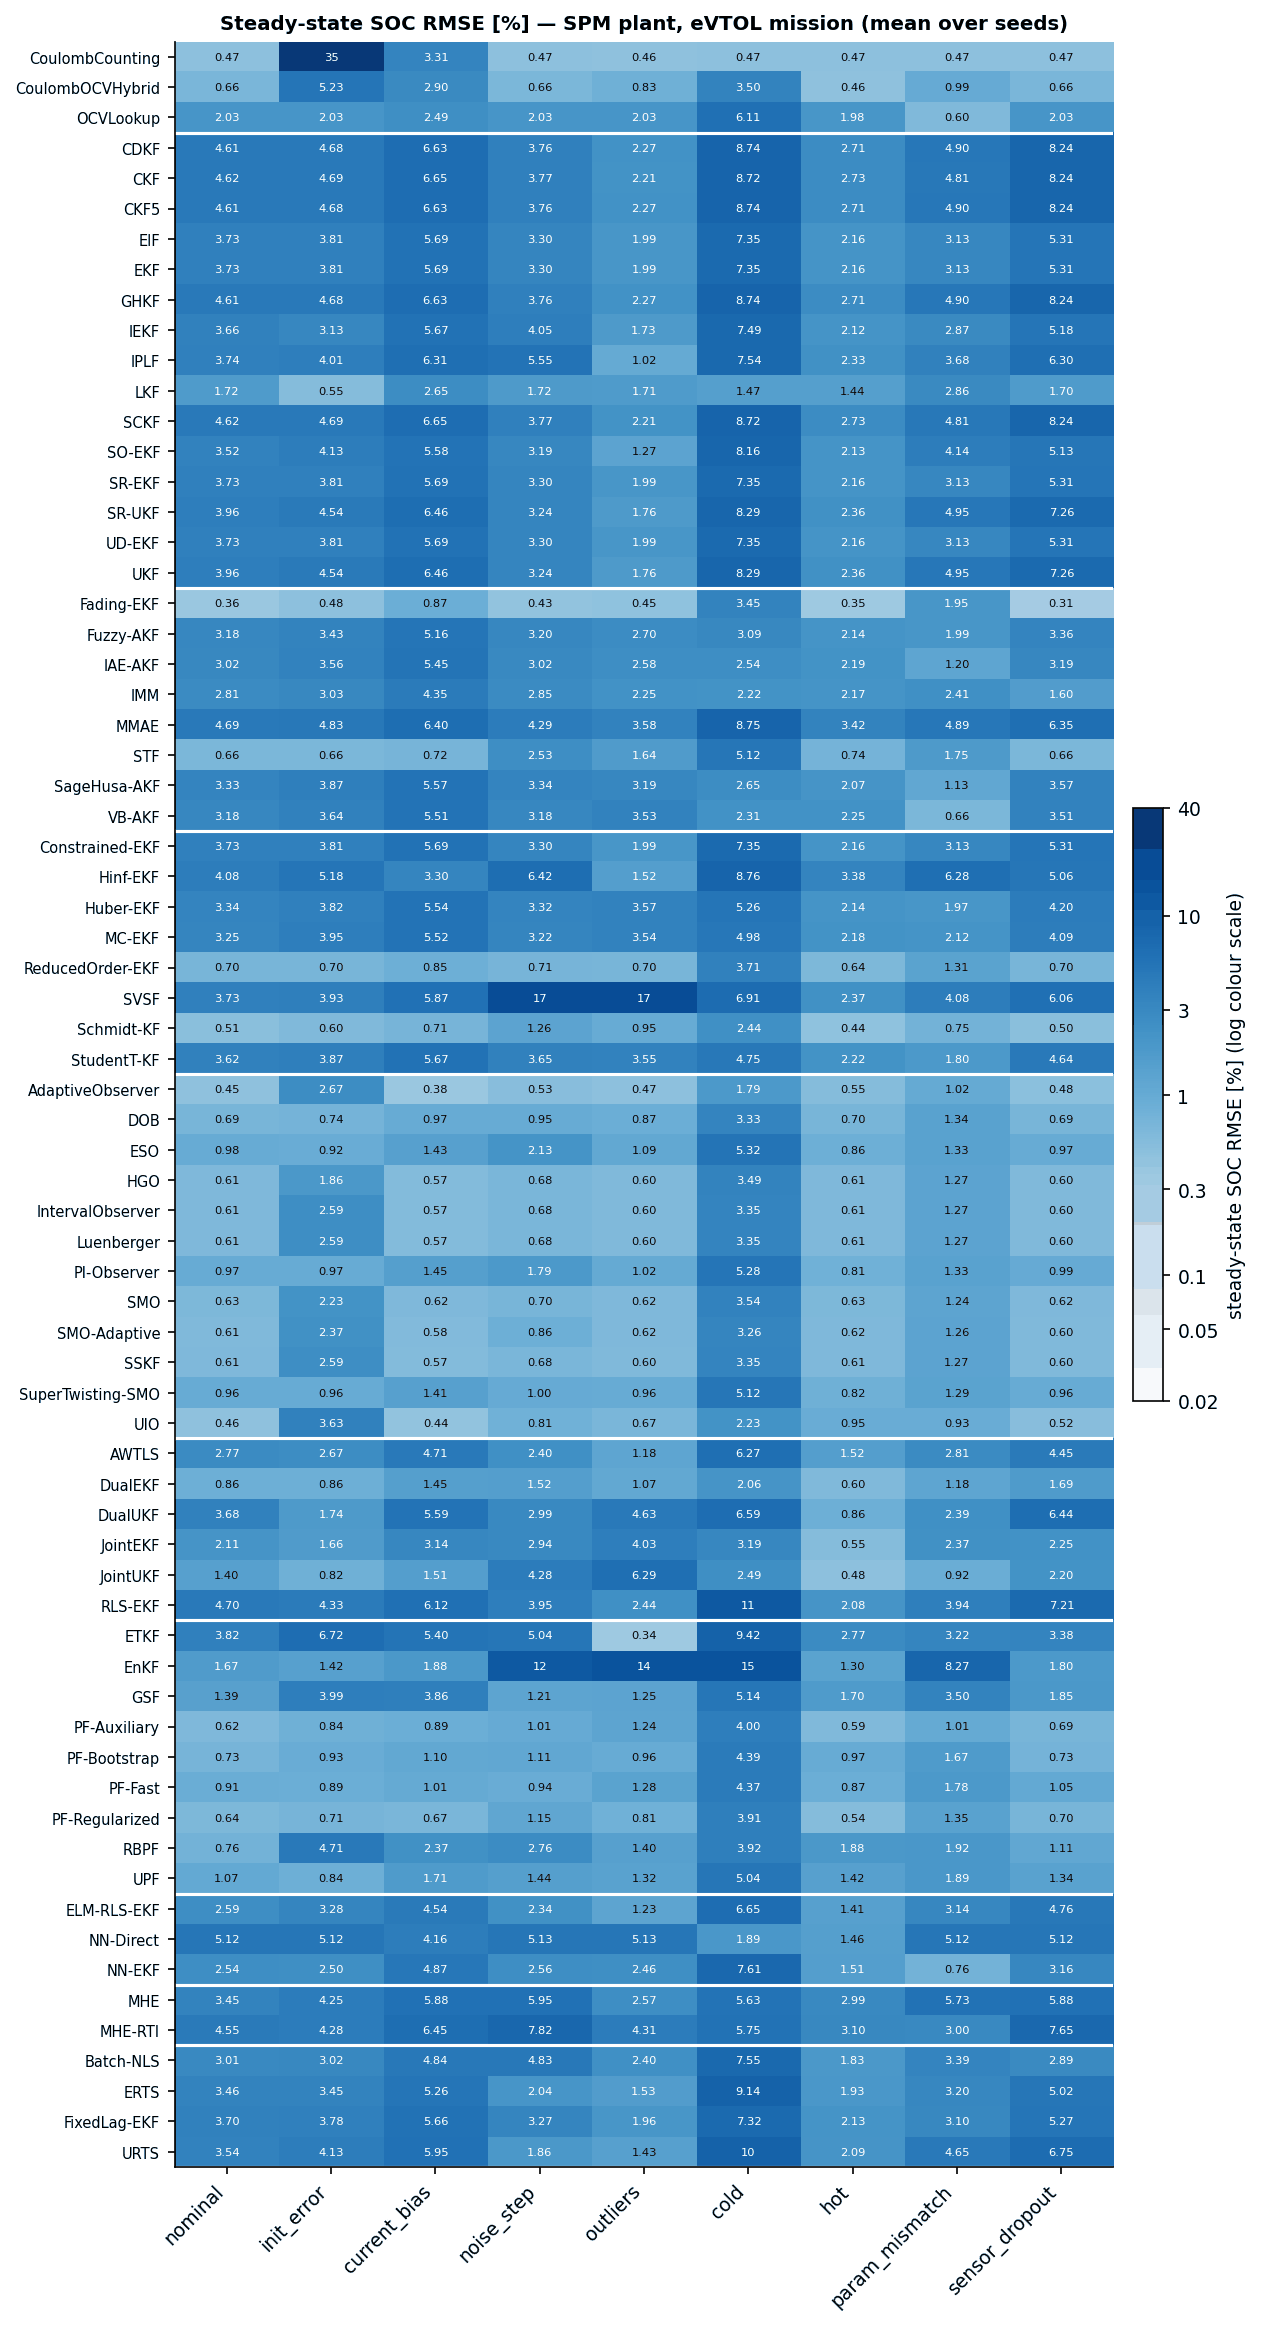
\includegraphics[width=0.98\textwidth]{figures/overview_heatmap_spm.png}
\caption{Steady-state SOC RMSE on the electrochemical plant as a heat map. Compared with
\cref{fig:res-heat-ecm} the picture is inverted: the rows that were uniformly light on the
equivalent-circuit plant --- the converged Kalman filters --- are now uniformly dark, and the
lightest rows belong to the fixed-gain observers, the fading-memory filter, the Schmidt filter
and the particle filters.}
\label{fig:res-heat-spm}
\end{figure}

\section{The inversion}

The headline result is the one that \cref{fig:res-ecm-vs-spm} shows: the nominal accuracy on the
two plants is uncorrelated across the library. The estimators that sit on the sensor-noise
floor of the equivalent-circuit plant --- the EKF and its algebraic equivalents, the
sigma-point and cubature filters, the $\mR$-adapting and M-estimator filters, the smoothers,
MHE --- form a cluster at \num{2.6}--\num{4.7}\,\% on the electrochemical plant, with a median
of \num{3.7}. The estimators that were mediocre on the equivalent circuit because they trust
the voltage less --- the Schmidt filter (\num{0.51}), the reduced-order EKF (\num{0.70}), the
strong-tracking filter (\num{0.66}), every fixed-gain observer (\num{0.45}--\num{0.98}) --- are
now the best of the field, and the fading-memory EKF, 12th on the equivalent circuit, is first
at \num{0.36}. The composite ranking over the nine scenarios reads, from the top, Fading-EKF
(geometric mean \num{0.65}), adaptive observer (\num{0.72}), Schmidt--Kalman (\num{0.78}),
UIO and HGO (\num{0.91}), reduced-order EKF (\num{0.92}), then Coulomb counting, the
regularised particle filter and the Luenberger group at \num{0.94}; the EKF is at \num{3.7},
the third-degree cubature family at \num{4.7}, MHE-RTI at \num{4.9} and the SVSF, which
diverges in one seed of \code{outliers}, at \num{6.0}.

\begin{figure}[H]\centering
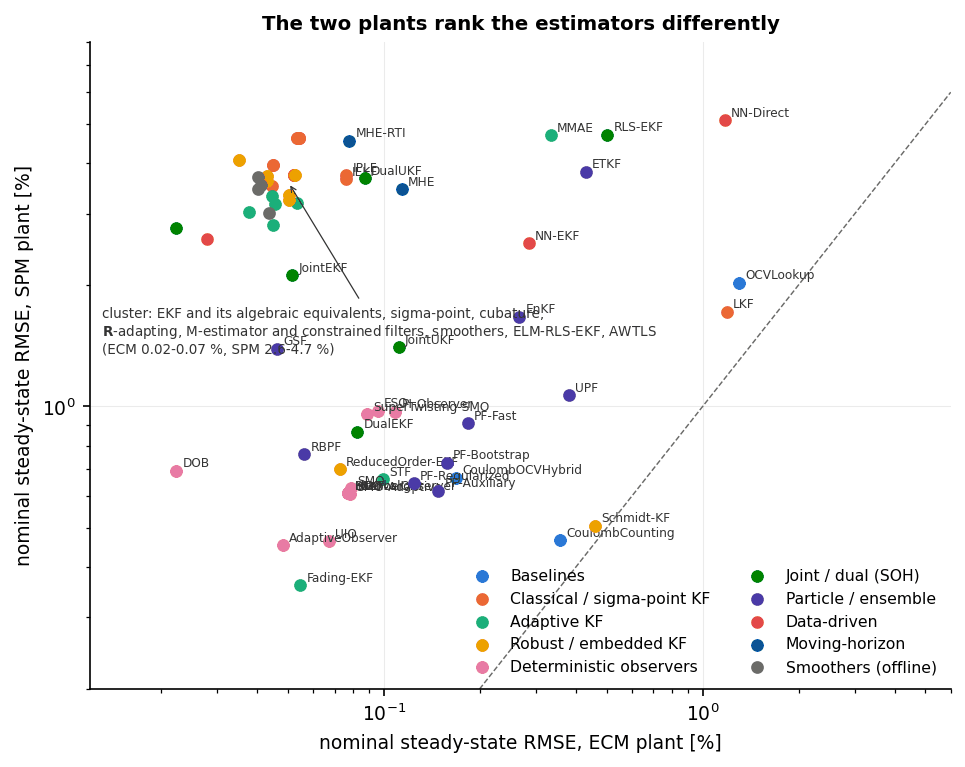
\includegraphics[width=0.9\textwidth]{figures/res_ecm_vs_spm.png}
\caption{Nominal steady-state RMSE on the equivalent-circuit plant against the same quantity on
the electrochemical plant, one point per estimator. The dashed line is equality. There is no
correlation: the cluster of converged Kalman-type filters is twenty times worse on the
electrochemical plant than on the equivalent circuit, while the fixed-gain observers and the
fading-memory filter lose a factor of five to eight and end up an order of magnitude ahead.}
\label{fig:res-ecm-vs-spm}
\end{figure}

\section{What happens, sample by sample}

\Cref{fig:res-spm-traces} plots the SOC error of eight estimators on the nominal mission. Up to
the take-off hover at \SI{3}{\minute} all of them agree to within half a percent and their
voltage residuals are the same \SIrange{1}{4}{\milli\volt}. At the hover the current rises to
\SIrange{21}{32}{\ampere} and the fitted circuit stops being a model of the cell: its fast branch
charges in \SI{15}{\second}, faster than the surface concentration of the particles depletes, and
its slow branch, with $\tau_2 = \SI{556}{\second}$, relaxes on the wrong time scale afterwards.
The open-loop residual of the circuit evaluated at the true state --- the quantity that Coulomb
counting reports as its voltage prediction error --- swings from \SI{-28}{\milli\volt} twenty
seconds into the hover to \SI{+30}{\milli\volt} a minute after it, and stays above
\SI{20}{\milli\volt} for the following two minutes. The estimators split on how they absorb
that swing. The EKF meets it with a covariance shaped by ninety seconds of confident updates:
an SOC standard deviation of \num{0.35}\,\% and cross-covariances with the RC states that
encode the circuit's own statement of which state combinations the voltage cannot
distinguish. The first three seconds of the hover move its SOC down by \num{3.6}\,\%, the standard
deviation falls to \num{0.21}\,\%, the innovation returns to within a few millivolts, and the
filter is from then on in a self-consistent state: the wrong SOC, compensated by the other
states of the circuit, fits the voltage to within the declared measurement noise, and with a
gain sized for a \num{0.2}\,\% prior nothing in the cruise data moves it back. The error is
still \num{-4.0}\,\% at \SI{20}{\minute} and \num{-3.6}\,\% at landing. The UKF and MHE follow
the same path to \num{-3.6} and \num{-3.7}\,\%.

The fading-memory filter makes the same excursion, to \num{-1.3}\,\%, but its covariance is
bounded below by construction, so the cruise residual, small as it is, pulls the estimate back
to half a percent within five minutes; the Luenberger observer, whose gain never changed,
overshoots to \num{-2.4}\,\% and recovers in the same way; the Schmidt filter is held near
\num{-1}\,\% by the inflated innovation covariance of its consider parameters and drifts to
\num{+0.7}\,\% by the end; the dual EKF re-identifies its parameters and crosses zero after
\SI{25}{\minute}. Coulomb counting, which does not look at the voltage, drifts from \num{0}
to \num{-0.6}\,\% under the current-sensor bias and is, at \num{0.47}\,\% steady state, the
fourth-best estimator on this plant --- a fact that says more about the plant than about
Coulomb counting.

\begin{figure}[H]\centering
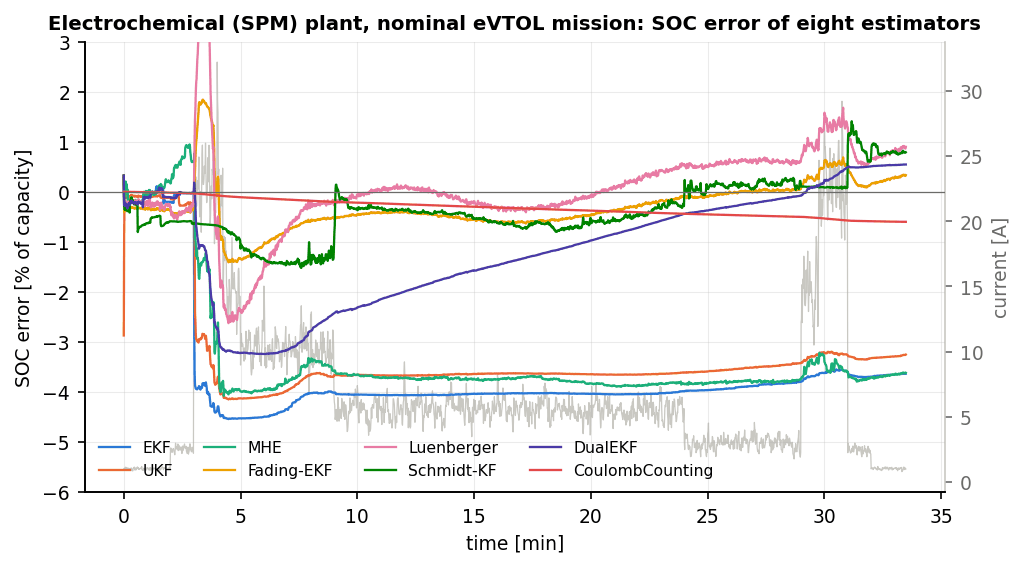
\includegraphics[width=\textwidth]{figures/res_spm_traces.png}
\caption{SOC error of eight estimators on the electrochemical plant, nominal eVTOL mission,
seed~1. The take-off hover at \SI{3}{\minute} creates the error; what distinguishes the
estimators is whether their gain is still large enough afterwards to remove it.}
\label{fig:res-spm-traces}
\end{figure}

Two consequences deserve to be stated as rules. First, on a plant with structured model
error the voltage residual is not an indicator of SOC accuracy: the EKF's residual is
\SI{1.0}{\milli\volt} RMS with a \num{3.7}\,\% SOC error, Coulomb counting's is
\SI{10}{\milli\volt} with \num{0.47}\,\%, and the Schmidt filter's is \SI{7.5}{\milli\volt}
with \num{0.51}\,\%. A BMS that monitors its own health through the innovation sequence will
report the EKF as healthy in this situation. Second, the optimal filter for a wrong model is
confidently wrong. The EKF is not failing here because of linearisation error --- the UKF and
the cubature filters, which linearise statistically, are worse, not better --- but because it
computes the exact posterior of a model whose measurement equation does not describe the
cell during a \SI{6}{C} pulse, and the posterior of a wrong model has no reason to be centred
on the truth.

\section{Column by column}

\paragraph{\code{init\_error}.} The observers, which take \SIrange{320}{350}{\second} to remove
a \num{0.35} initial error on the equivalent-circuit plant, take about as long here and are
therefore worse than their nominal figures (\num{1.9}--\num{3.6}\,\%); the Kalman filters
remove the initial error in one sample as before and their column is their nominal bias. The
fading-memory EKF (\num{0.48}), the Schmidt filter (\num{0.60}), the regularised particle
filter (\num{0.71}), the disturbance observer (\num{0.74}) and the joint UKF (\num{0.82}) are
the estimators that do both --- converge quickly and not park on the hover bias.

\paragraph{\code{current\_bias}.} The state-only Kalman filters add the unobservable bias
error to their hover bias and read \num{5.5}--\num{6.7}\,\%; the estimators that stay close to
the voltage are at \num{0.4}--\num{0.9}\,\% (adaptive observer \num{0.38}, UIO \num{0.44},
HGO and Luenberger \num{0.57}, Schmidt \num{0.71}, STF \num{0.72}, Fading-EKF \num{0.87}),
because on this plant the voltage is the reliable signal and a high gain on it is exactly
what a current-sensor bias calls for. MHE, the best estimator in this column on the
equivalent circuit, is at \num{5.9}\,\% here: its window re-fits a model that is wrong in
the same way at every node.

\paragraph{\code{noise\_step} and \code{outliers}.} The robust and adaptive filters that won
these columns on the equivalent circuit are now in the cluster (\num{3.2}--\num{3.7} and
\num{2.5}--\num{3.6}\,\%), because raising $\mR$ in response to the residual lowers the gain,
and a lower gain is the wrong direction on this plant; their sensor-fault handling is intact
but is masked by the model error. The estimators that handle the fault without lowering their
gain on SOC --- the fixed-gain observers (\num{0.53}--\num{1.0}), the fading-memory filter
(\num{0.43}/\num{0.45}), the reduced-order EKF (\num{0.71}/\num{0.70}), the particle filters
(\num{0.8}--\num{1.3}) --- keep their nominal accuracy. The IPLF (\num{1.02} on
\code{outliers}) and the ETKF (\num{0.34}) are the exceptions within their families; the SVSF
diverges in one seed of \code{outliers} and the EnKF in two seeds of \code{cold}.

\paragraph{\code{cold}.} At \SI{-10}{\celsius} the diffusion time constant of the plant grows by
an order of magnitude and the hover residual with it; this is the hardest column of the table,
with a median of \num{5.2}\,\% and no estimator below \num{1.5}\,\% except the linear Kalman
filter (\num{1.47}), whose frozen gain happens to be right for a cell this slow, and the
adaptive observer (\num{1.79}). The IMM (\num{2.22}), VB-AKF (\num{2.31}), UIO (\num{2.23}),
Schmidt (\num{2.44}) and the $\mR$-adapting filters (\num{2.5}--\num{2.7}) follow; the EKF
reads \num{7.35}, the cubature filters \num{8.7}, the EnKF diverges. On a cold
electrochemical cell the 2-RC circuit is simply not a model of the voltage under load, and
the estimator choice moves the error by a factor of three, not by an order of magnitude.

\paragraph{\code{hot}.} The mirror image: at \SI{45}{\celsius} diffusion is fast, the hover
residual shrinks and every estimator improves, the cluster to \num{2.1}--\num{2.4}\,\% and the
observers, the Fading-EKF, the Schmidt filter and the particle filters to \num{0.35}--\num{0.65}.

\paragraph{\code{param\_mismatch} and \code{sensor\_dropout}.} A parameter error on top of a
structural error is mostly absorbed by the estimators that already discount the model
(VB-AKF \num{0.66}, Schmidt \num{0.75}, NN-EKF \num{0.76}, joint UKF \num{0.92}, UIO
\num{0.93}), and the plain Kalman filters read \num{3.1}--\num{4.9}. The stuck voltage channel
is handled as on the equivalent circuit, with the same family ordering, on top of the hover
bias: Fading-EKF \num{0.31}, adaptive observer \num{0.48}, Schmidt \num{0.50}, the observer
group \num{0.6}--\num{1.0}, the EKF \num{5.31}, the cubature filters \num{8.24}.

\section{What the electrochemical results say}

The benchmark makes three points that are easy to state and easy to forget.

The estimator that is best for the model is not the estimator that is best for the cell. On
a plant whose physics the estimator's model cannot reproduce, the Bayesian-optimal filters
are the worst group in the table and the estimators that were designed with model error in
mind --- fading memory, consider parameters, fixed gains, particle clouds with roughening ---
are the best. A practitioner who selects an estimator on an equivalent-circuit simulation, or
on a real cell under gentle excitation, will select the wrong one for a cell that sees
\SI{6}{C} pulses.

The remedy is not a better filter but a better model, or a filter that knows its model is
wrong. Every estimator in the table runs the same identified circuit; the \num{0.36}\,\% of
the fading-memory filter is what that circuit can deliver when the estimator refuses to let
one transient decide the rest of the flight. A reduced electrochemical model in the estimator
--- a single-particle model with a few diffusion states, which the library's model concept
admits without change --- would remove the structured residual at its source, and is the
first item of future work in \cref{ch:res-conclusions}.

Health monitoring must not rely on the innovation alone. Under structured model error a
converged filter reports a clean innovation and a wrong state. A second, independent
estimate --- Coulomb counting, an OCV reading at rest, a high-gain observer running in
parallel --- is the only way to detect the discrepancy, and \cref{ch:res-recommendations}
makes that a design rule.
